

\begin{itemize}
    
    \item Análisis del problema:
    
     El sistema de control de acceso tiene como propósito verificar una contraseña digital ingresada mediante una combinación de botones físicos o un teclado matricial. Si la combinación es correcta, se activa una cerradura electrónica (servo motor o relé); en caso contrario, se contabilizan los intentos fallidos y, al superar el límite permitido, el sistema entra en un estado de bloqueo temporal.
     
        \begin{itemize}
             \item Identificación de Entradas y Salidas
                  \begin{itemize}       
                      \item Entradas del sistema:
                    
                            \begin{itemize}
                                 \item  Botones digitales (4 pulsadores) o teclado matricial 4x4 para ingreso de contraseña.

                                 \item Señal de reset (opcional): botón para reiniciar el sistema desde estado bloqueado.                      
                             \end{itemize}  
                             
                  \end{itemize}     

             \item Restricciones Técnicas
                     \begin{itemize}
                            \item Máximo 3 intentos fallidos antes de activar el bloqueo.
                            
                            \item Tiempo de bloqueo: 30 segundos.

                            \item La contraseña debe almacenarse en memoria no volátil (EEPROM) o en código.
                            
                            \item Temporización no bloqueante mediante millis()

                            \item El sistema debe retornar automáticamente al estado de espera tras el desbloqueo.
                     \end{itemize}
                     
             \item Variables Involucradas
                 
\begin{table}[h]
\centering
\caption{Variables del sistema de control de acceso}
\label{tab:Tabla_1_R1}
\footnotesize
\setlength{\tabcolsep}{4pt}
\renewcommand{\arraystretch}{1.5}
    
    \begin{tabularx}{\columnwidth}{|>{\raggedright\arraybackslash}p{3cm}|>{\centering\arraybackslash}p{1.5cm}|X|}
        \hline
        \textbf{Variable} & \textbf{Tipo} & \textbf{Descripción} \\
        
        \hline
        intentosFallidos & int & Contador de intentos incorrectos (0--3) \\ 
        
        \hline
        contrasenaIngresada & String & Secuencia de teclas presionadas por el usuario \\ 
        
        \hline
        contrasenaCorrecta & String & Contraseña almacenada en firmware \\ 
        
        \hline
        sistemaBloqueado & bool & Indica si el sistema está en estado de bloqueo \\ 
        
        \hline
        tiempoBloqueo & unsigned long & Marca de tiempo de inicio del bloqueo \\ 
        
        \hline
        accesoGarantizado & bool & Indicador de acceso concedido \\ \hline
\end{tabularx}
\end{table}
          
       \end{itemize}  
\end{itemize}


\begin{itemize}

       \item Flujograma del sistema
       
         A continuación se describe el algoritmo de comportamiento del sistema de control de acceso. El diagrama representa el flujo lógico completo desde el inicio hasta la resolución de cada evento de acceso.

             \begin{itemize}
             
                \item Descripción del Algoritmo (Pseudocódigo Estructurado):

                En el Algoritmo~\ref{alg:Algoritmo1} se puede observar el pseudocódigo, el cual, comienza declarando un bloque de INICIO que configura los periféricos. A continuación se evalúa si el sistema está bloqueado; en caso afirmativo, se verifica el temporizador y se libera al cumplirse 30 segundos. Si el sistema no está bloqueado, se espera la entrada del usuario. Cuando la contraseña está completa, se ejecuta la comparación: si es correcta, se activa el servo y el LED verde; si es incorrecta, se incrementa el contador de fallos y se evalúa si se alcanzó el límite. El proceso retorna al inicio del bucle en todos los casos.

                  
             \end{itemize}
             
\end{itemize}

\begin{algorithm}[h]
\caption{Algoritmo de Control de Acceso}
\label{alg:Algoritmo1}
\begin{algorithmic}[1]

\Statex \textbf{Inicialización:}
\State Inicializar pines, variables y servo en posición cerrada
\State $intentosFallidos = 0$
\State $sistemaBloqueado = false$

\While{true}

    \If{$sistemaBloqueado$}

        \If{$millis() - tiempoBloqueo \geq 30000$}
            \State $sistemaBloqueado = false$
            \State $intentosFallidos = 0$
            \State Apagar $LED\_ROJO$
        \EndIf

    \Else

        \State Leer tecla del teclado
        \State Agregar caracter a $contrasenaIngresada$

        \If{$|contrasenaIngresada| = |contrasenaCorrecta|$}

            \If{$contrasenaIngresada = contrasenaCorrecta$}

                \State Activar servo (abrir cerradura)
                \State Encender $LED\_VERDE$ durante 3 segundos
                \State Regresar servo a posicion cerrada
                \State $intentosFallidos = 0$

            \Else

                \State $intentosFallidos = intentosFallidos + 1$
                \State Hacer parpadear $LED\_ROJO$

                \If{$intentosFallidos \geq 3$}
                    \State $sistemaBloqueado = true$
                    \State $tiempoBloqueo = millis()$
                \EndIf

            \EndIf

            \State $contrasenaIngresada = " "$

        \EndIf

    \EndIf

\EndWhile

\end{algorithmic}
\end{algorithm} 
%\bigskip


\begin{itemize}

    \item Justificación técnica del microcontrolador seleccionado

        \begin{itemize}

             \item Microcontrolador Seleccionado: Arduino UNO (ATmega328P): El Arduino UNO con microcontrolador ATmega328P resulta adecuado para este sistema debido a su disponibilidad, bajo costo, amplia comunidad de soporte y suficiente cantidad de pines para los periféricos requeridos\cite{Arduino_datasheet}.

             \item Análisis de Pines Requeridos:
              El ATmega328P dispone de 14 pines digitales (6 con PWM) y 6 analógicos, cubriendo ampliamente los 12 pines requeridos con margen de expansión.
              
                 

\begin{table}[h]
\caption{Análisis de Pines Requeridos}
\label{tab:Tabla_2_R1}
\centering
\renewcommand{\arraystretch}{1.2}
\begin{tabular}{p{2.5cm} p{3.5cm} p{2cm}}
\toprule
\textbf{Componente} & \textbf{Pines Requeridos} & \textbf{Tipo} \\
\midrule
Teclado matricial 4x4 & 8 pines digitales (4 filas + 4 columnas) & Digital I/O \\
LED verde & 1 pin digital & Digital OUTPUT \\
LED rojo & 1 pin digital & Digital OUTPUT \\
Servo motor & 1 pin PWM & PWM OUTPUT \\
Buzzer & 1 pin digital & Digital OUTPUT \\
\midrule
\textbf{Total} & \textbf{12 pines} & --- \\
\bottomrule
\end{tabular}
\end{table}

             \item Capacidad de Procesamiento

                 \begin{itemize}
                 
                       \item CPU: ATmega328P @ 16 MHz
                       \item Memoria Flash: 32 KB (programa ocupa < 5 KB)
                       \item SRAM: 2 KB (suficiente para buffers de contraseña y variables de estado)
                       \item EEPROM: 1 KB (almacenamiento persistente de contraseña) 
                       
                 \end{itemize}

             \item Consumo Energético

                  \begin{itemize}
                 
                       \item Consumo activo: ~46 mA @ 5V = ~230 mW
                       \item LED: ~20 mA c/u con resistencia limitadora de 220 ohms
                       \item Servo SG90: ~100–250 mA en movimiento
                       \item Alimentación recomendada: 5V/1A (USB o adaptador)
                       
                 \end{itemize}
                 
             \item Componentes Auxiliares
                  \begin{table}[h]
\caption{Componentes Electrónicos del Sistema}
\label{tab:Tabla_3_R1}
\centering

\footnotesize
\setlength{\tabcolsep}{4pt}
\renewcommand{\arraystretch}{1.5}

\begin{tabularx}{\columnwidth}{|>{\raggedright\arraybackslash}p{3cm}|>{\centering\arraybackslash}p{1.5cm}|X|}
\hline
\textbf{Componente} & \textbf{Cant.} & \textbf{Especificación / Función} \\
\hline
LED verde 5mm & 1 & 3.3V, 20mA. Indicador de acceso correcto. \\
\hline
LED rojo 5mm & 1 & 3.3V, 20mA. Indicador de error o bloqueo. \\
\hline
Resistencia 220 $\Omega$ & 2 & 1/4 W. Limitación de corriente para los LEDs. \\
\hline
Buzzer pasivo & 1 & 5V. Generación de señal sonora de retroalimentación. \\
\hline
Protoboard / PCB & 1 & 830 puntos. Montaje físico del circuito. \\
\hline
\end{tabularx}

\end{table}

             \item Esquema de Conexión

             En la Figura \ref{fig:Imagen_1_R1} se observa el diagrama de conexión correspondiente al funcionamiento de este circuito, desarrollado a través del programa de circuitado. A continuación se mencionan las conexiones establecidas en el proyecto:
             \begin{itemize}
                 \item Teclado 4x4: Filas a pines D4, D5, D6, D7 — Columnas a pines D8, D9, D10, D11
                \item LED verde: Pin D12 → Resistencia 220 ohms → Ánodo LED → Cátodo → GND
                \item LED rojo: Pin D13 → Resistencia 220 ohms → Ánodo LED → Cátodo → GND
                \item Servo SG90: Cable señal a Pin D3 (PWM), VCC a 5V, GND a GND
                \item Buzzer: Pin D2 → Buzzer (+) → GND
                \item Alimentación: 5V desde USB o regulador 7805

             \end{itemize}
             \textit{EasyEDA}.
                  \begin{figure}[h]
                  \centering
                  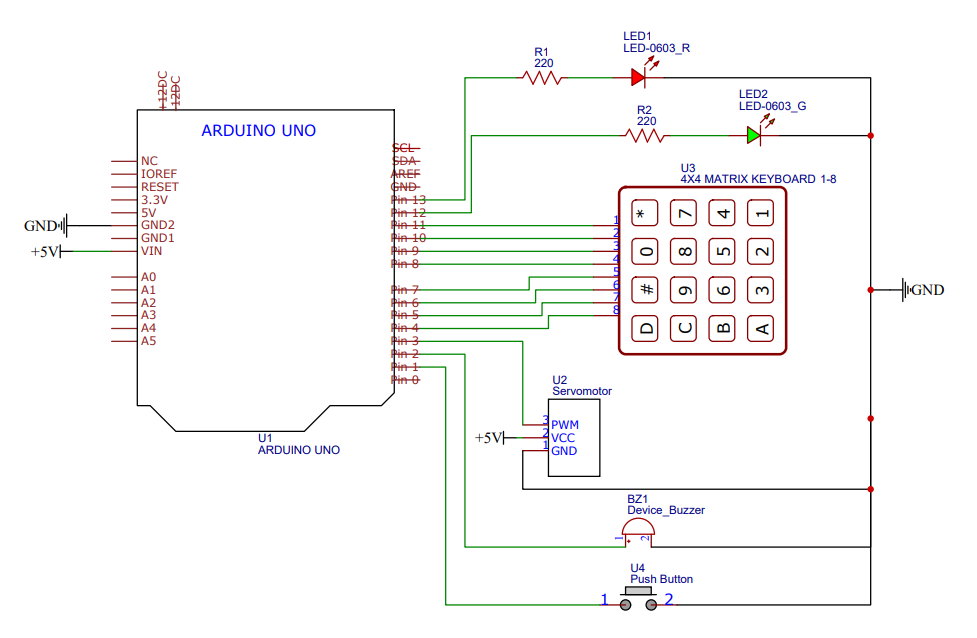
\includegraphics[width=\columnwidth]{images/Imagen_1R1.png}
                  \caption{Esquemático de Conexión Reto 1}
                  \label{fig:Imagen_1_R1}
                  \end{figure}
             
        \end{itemize}
  
\end{itemize}

\begin{itemize}
      \item Código documentado
      
      El código está organizado de forma modular separando la inicialización de hardware, la lógica de verificación, el control de la cerradura y la gestión de estados de bloqueo. Se evita el uso de delay() para garantizar temporización no bloqueante.

      \begin{lstlisting}[caption={Implementación de Control de Acceso con Teclado y Servo}, label={lst:control-acceso}]
#include <Keypad.h>
#include <Servo.h>

// --- Definicion de pines ---
#define PIN_SERVO       3
#define PIN_BUZZER      2
#define PIN_LED_VERDE   12
#define PIN_LED_ROJO    13
#define PIN_BOTON       A0

// --- Configuracion del teclado 4x4 ---
const byte FILAS    = 4;
const byte COLUMNAS = 4;

char teclas[FILAS][COLUMNAS] = {
  { '1', '2', '3', 'A' },
  { '4', '5', '6', 'B' },
  { '7', '8', '9', 'C' },
  { '*', '0', '#', 'D' }
};

byte pinesFilas[FILAS] =
  { 11, 10, 9, 8 };
byte pinesColumnas[COLUMNAS] =
  {  7,  6, 5, 4 };

Keypad teclado =
  Keypad(makeKeymap(teclas),
         pinesFilas,
         pinesColumnas,
         FILAS,
         COLUMNAS);

// --- Servo ---
Servo servo;
#define ANGULO_ABIERTO  90
#define ANGULO_CERRADO   0

// --- Variables de control de 
acceso ---
const String PASSWORD = "1234";
const byte MAX_INTENTOS = 3;
const unsigned long TIEMPO_BLOQUEO
= 30000;

// --- Estado general ---
String entradaActual = "";
byte intentosFallidos = 0;
bool bloqueado = false;
unsigned long tiempoBloqueo = 0;

// --- Servo temporizado ---
bool puertaAbierta = false;
unsigned long tiempoServo = 0;

// --- Buzzer no bloqueante ---
bool buzzerActivo = false;
unsigned long tiempoBeep = 0;
int duracionBeep = 0;

// --- Parpadeo LED rojo ---
unsigned long tiempoBlink = 0;
bool estadoBlink = false;
byte parpadeosPendientes = 0;
bool ledRojoFijo = false;

// --- Anti-rebote boton ---
unsigned long ultimoDebounce = 0;
const unsigned long 
DEBOUNCE_DELAY = 50;

// ===================
void inicializarHardware() {
  pinMode(PIN_LED_VERDE, OUTPUT);
  pinMode(PIN_LED_ROJO, OUTPUT);
  pinMode(PIN_BUZZER, OUTPUT);
  pinMode(PIN_BOTON, 
  INPUT_PULLUP);
  servo.attach(PIN_SERVO);
  servo.write(ANGULO_CERRADO);
  digitalWrite(PIN_LED_VERDE, LOW);
  digitalWrite(PIN_LED_ROJO,  LOW);
  Serial.println("Sistema de
  acceso listo");
}

// ===================
void beep(int frecuencia,
          int duracion) {
  tone(PIN_BUZZER, frecuencia);
  buzzerActivo = true;
  tiempoBeep   = millis();
  duracionBeep = duracion;
}

// ===================
void actualizarBuzzer() {
  if (buzzerActivo) {
    if (millis() - tiempoBeep
        >= duracionBeep) {
      noTone(PIN_BUZZER);
      buzzerActivo = false;
    }
  }
}

// ===================
void actualizarServo() {
  if (puertaAbierta) {
    if (millis() - tiempoServo
        >= 3000) {
      servo.write(ANGULO_CERRADO);
      digitalWrite(PIN_LED_VERDE,
      LOW);
      puertaAbierta = false;
    }
  }
}

// ===================
void actualizarBlink() {
  if (!estadoBlink) return;
  if (millis() - tiempoBlink < 300)
    return;
  tiempoBlink = millis();
  bool ledActual =
    digitalRead(PIN_LED_ROJO);
  if (!ledActual) {
    digitalWrite(PIN_LED_ROJO, HIGH);
    parpadeosPendientes--;
  } else {
    if (parpadeosPendientes == 0) {
      estadoBlink = false;
      digitalWrite(PIN_LED_ROJO,
        ledRojoFijo ? HIGH : LOW);
    } else {
      digitalWrite(PIN_LED_ROJO, LOW);
    }
  }
}

// ===================
void accesoAprobado() {
  intentosFallidos  = 0;
  estadoBlink       = false;
  ledRojoFijo       = false;
  digitalWrite(PIN_LED_ROJO,  LOW);
  digitalWrite(PIN_LED_VERDE, HIGH);
  servo.write(ANGULO_ABIERTO);
  puertaAbierta = true;
  tiempoServo   = millis();
  beep(2000, 150);
}

// ===================
void accesoNegado() {
  intentosFallidos++;
  if (intentosFallidos < 
  MAX_INTENTOS)
  {
    parpadeosPendientes = 2;
    ledRojoFijo         = false;
  } else {
    parpadeosPendientes = 3;
    ledRojoFijo         = true;
  }
  estadoBlink = true;
  tiempoBlink = millis();
  digitalWrite(PIN_LED_ROJO, LOW);
  beep(500, 500);
  if (intentosFallidos >= 
  MAX_INTENTOS)
  {
    bloqueado     = true;
    tiempoBloqueo = millis();
  }
}

// ===================
void verificarPassword() {
  if (entradaActual == PASSWORD)
    accesoAprobado();
  else
    accesoNegado();
  entradaActual = "";
}

// ===================
void procesarTecla(char tecla) {
  if (tecla == '#') {
    verificarPassword();
    return;
  }
  if (tecla == '*') {
    entradaActual = "";
    beep(1000, 100);
    return;
  }
  entradaActual += tecla;
  if (entradaActual.length()
      > PASSWORD.length()) {
    entradaActual = "";
    beep(500, 200);
  }
}

// ===================
void leerBoton() {
  if (digitalRead(PIN_BOTON) == LOW) {
    if (millis() - ultimoDebounce
        > DEBOUNCE_DELAY) {
      bloqueado        = false;
      intentosFallidos = 0;
      entradaActual    = "";
      estadoBlink      = false;
      ledRojoFijo      = false;
      digitalWrite(PIN_LED_ROJO, LOW);
      digitalWrite(PIN_LED_VERDE, 
      LOW);
      beep(1800, 200);
      ultimoDebounce = millis();
    }
  }
}

// ===================
void setup() {
  Serial.begin(9600);
  inicializarHardware();
}

// ===================
void loop() {
  actualizarBuzzer();
  actualizarServo();
  actualizarBlink();
  leerBoton();
  if (bloqueado) {
    if (millis() - tiempoBloqueo
        >= TIEMPO_BLOQUEO) {
      bloqueado        = false;
      intentosFallidos = 0;
      estadoBlink      = false;
      ledRojoFijo      = false;
      digitalWrite(PIN_LED_ROJO, LOW);
      beep(1500, 300);
    }
    return;
  }
  char tecla = teclado.getKey();
  if (tecla) procesarTecla(tecla);
}
\end{lstlisting}
      
\end{itemize}

